\subsection{Problem 3.6. Managing Road Checkpoints}

\paragraph{}
\begin{quote}
Two large cities X and Y are located on different sides of the state border. The region between X and Y is highly urbanized. The official customs post between the two states is abolished some time ago. However, the governments of both states want to get an idea of the commodity flows from X to Y. To that end they want to open a number of checkpoints along the roads that are used when traveling from X to Y. The road map with the relevant road segments is depicted in Figure \ref{network3-6}. After careful examination of the commodity flows, it is decided that vehicles traveling only in one direction will be checked, besides the fact that in this heavily urbanized region already many roads are one-way. The road segments and their directions are depicted in Figure 3.16. There is a total of 47 junctions. GTC has obtained the order to build the communication system between the checkpoints. The first question to be solved is the number and the location of the checkpoints. Since the budget for building the communication system is rather restricted and GTC only wants to build a high quality system, the number of checkpoints is rather crucial. Therefore, GTC and the contractor have decided to determine a minimum number of checkpoints that need to be built. One of the major conditions is that, given the directions of commodity flow, all vehicles that travel from X to Y can be checked. The costs for building each checkpoint and constructing the communication system is estimated at \texteuro 300,000.

The two governments want to know a minimum price for the construction of a reliable checking system.
\end{quote}

\begin{figure}[H]
	\centering
%	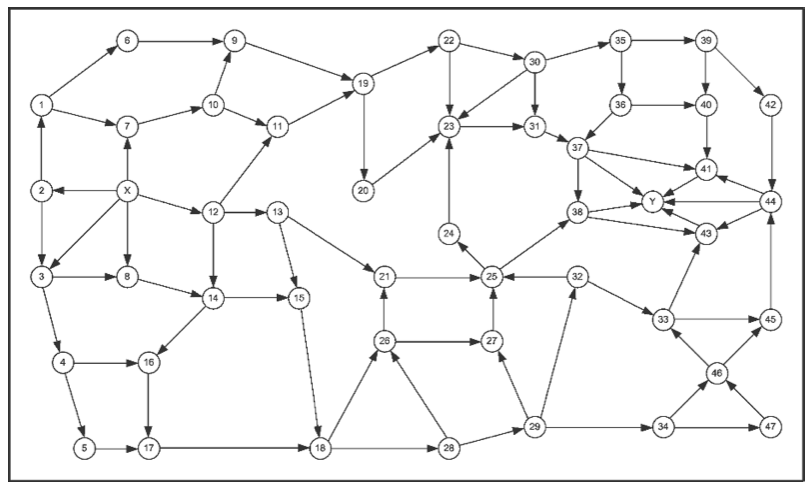
\includegraphics[scale=1]{./img/figure3-16.png}
	\caption{Road Map of the urbanized region of cities X and Y}
	\label{network3-6}
\end{figure}

